\section{Process' Perspective}
%\red{This perspective should clarify how code or other artifacts come from idea into the running system and everything that happens on the way.}

%\red{In particular, the following descriptions should be included:}

%\red{A complete description of stages and tools included in the CI/CD chains, including deployment and release of your systems.
%How do you monitor your systems and what precisely do you monitor?
%What do you log in your systems and how do you aggregate logs?
%Brief results of the security assessment and brief description of how did you harden the security of your system based on the analysis
%Applied strategy for scaling and upgrades
%In case you have used AI-assistants during your project briefly explain which system(s) you used during the project and reflect how it supported/hindered your process.}

This section provides an overview of the journey from idea to system, specifically detailing CI/CD chains, system monitoring, logging, security assessments, scaling and availability strategies, as well as the use of AI-assistants. %\textcolor{red}{er det fint med sådan en lille generic intro?}


%for this section see images/commit_checks,logging,monitor_bad,monitor_good
%https://codeclimate.com/github/TheisHS/test1-itu-minitwit -- link to codeclimate, everyone can see this
\subsection{CI/CD Pipeline}

\begin{figure}[H]
    \centering
    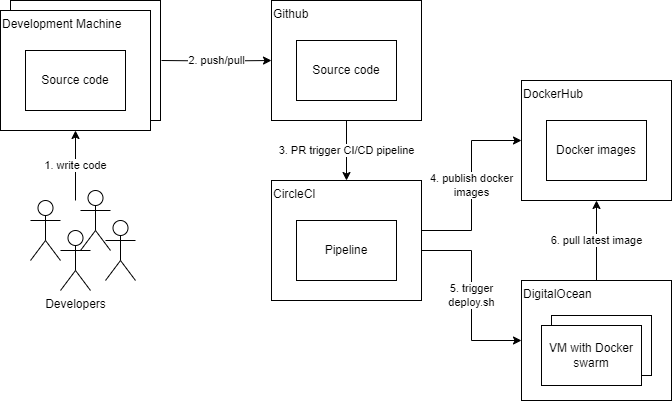
\includegraphics[width=0.7\textwidth]{images/cicd.png}
    \caption{Visualisation of the CI/CD pipeline.}
    \label{fig:cicd}
\end{figure}

Our pipeline for CI/CD is depicted in figure \ref{fig:cicd}. The source code on Github is linted by a CircleCI workflow on each commit, and is analysed by several of the tools mentioned in the section below when a pull request is opened. When a pull request is merged into main, our \texttt{build\_and\_deploy} workflow is triggered, which can be seen in figure \ref{fig:build_and_deploy}. Releases have been done manually on Github once every Thurday evening.



\begin{figure}[H]
    \centering
    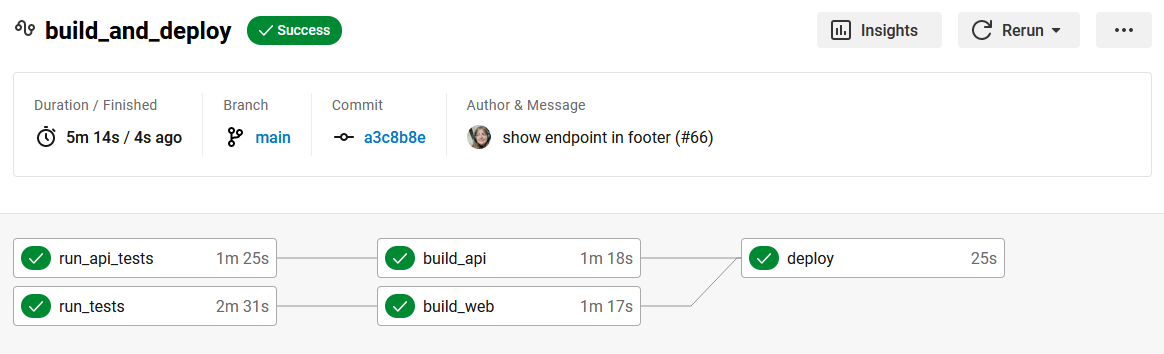
\includegraphics[width=\textwidth]{images/pipeline.png}
    \caption{The \texttt{build\_and\_deploy} workflow on CircleCI.}
    \label{fig:build_and_deploy}
\end{figure}

\subsubsection*{Tools and Technologies}
\begin{multicols}{2}
    \begin{itemize}
        \item \textbf{CircleCI}: A continuous integration and delivery platform that automates the build, test and deployment processes of our project. 
        \item \textbf{CodeClimate}: A platform that provides code review, offering insights into code quality, maintainability and test coverage, helping us ensure high standards and to improve code health.
        \item \textbf{Github}: Version Control Management
        \item \textbf{Hadolint}: A lint-tool that analyzes Dockerfiles to find common issues.
        \item \textbf{Shellcheck}: A shell script analysis tool that identifies syntax errors and common issues.
        \item \textbf{Sonarcloud}: A cloud-based code quality and security service that analyzes code to detect bugs and vulnerabilities.
        \item \textbf{Vagrant}: A tool for building and managing virtualized development environments. Used initially for VM instantiating.
    \end{itemize}
\end{multicols}

\subsubsection*{Technology choices}
The decision to manage our CI/CD pipeline on CircleCI is based on the pros and cons in appendix \ref{app:ci_tool_choice}. Github Actions would also have been a good choice for this, but as there were no obvious downsides to either or, we went with the technology that we had not work with before as to gain experience with it.



% \subsubsection*{Deployment and Release Processes}
% Docker, feb 29


\subsection{System Monitoring and Logging}

\subsubsection*{Monitoring Strategies and Tools}

%march 8,12,13 (check lecture notes for reactive vs proactive monitoring and what we have done)
In managing our system's health, we rely on two key tools: Prometheus and Grafana. Prometheus is a pull-based monitoring system that pulls/scrapes our defined metrics. We instrument the system with the Prometheus \textit{client\textunderscore golang} library, from which we create the metrics, register each metric using Prometheus' default register, finally creating a HTTP endpoint exposing the metrics endpoint for Prometheus to scrape \cite{prometheusGolang}. Our approach is mainly whitebox monitoring in application-based metrics tracking the internal workings of the system. However, we do use a few blackbox monitoring elements by tracking specific endpoint responses.

Grafana is an open-source platform used for visualising and analysing time-series data. In our setup, we use Grafana as a dashboarding tool that uses our Prometheus server as the primary data source for monitoring. This allows us to create dashboards that provide real-time insights of our measures.
%Reactive Monitoring: In reactive monitoring, the focus is on responding to issues after they occur.
%Proactive Monitoring: Proactive monitoring involves anticipating and preventing issues before they impact the system.

As from the Monitoring Maturity Model by James Turnbull \cite{MonitoringMaturityModel}, our monitoring strategy combines proactive elements, such as monitoring uptime and tracking error rates to anticipate and prevent issues, with reactive elements, such as tracking specific error codes and status of specific user requests to respond promptly to issues that arise.


\subsubsection*{Key Metrics Monitored}
We have defined monitoring metrics for both the API and the web client. However, given the API's consistent workload from the simulation, this has been our primary focus. We have defined a total of 14 metrics for the API:
\begin{multicols}{2}
\begin{itemize}
    \item \textbf{http\_requests\_total}
    \item \textbf{database\_accesses\_total}
    \item \textbf{errors\_total}
    \item \textbf{get\_user\_id\_requests}
    \item \textbf{get\_user\_id\_requests\_failed}
    \item \textbf{follow\_requests}
    \item \textbf{follow\_requests\_failed}
    \item \textbf{unfollow\_requests}
    \item \textbf{unfollow\_requests\_failed}
    \item \textbf{post\_message\_requests}
    \item \textbf{post\_message\_requests\_failed}
    \item \textbf{not\_found}
    \item \textbf{bad\_request}
    \item \textbf{internal\_server\_error}
\end{itemize}
\end{multicols}

These monitoring metrics are visualised in a Grafana dashboard named \texttt{Minitwit\_Dashboard} as shown in Figure \ref{fig:monitor_good}. 

\begin{figure}[H]
    \centering
    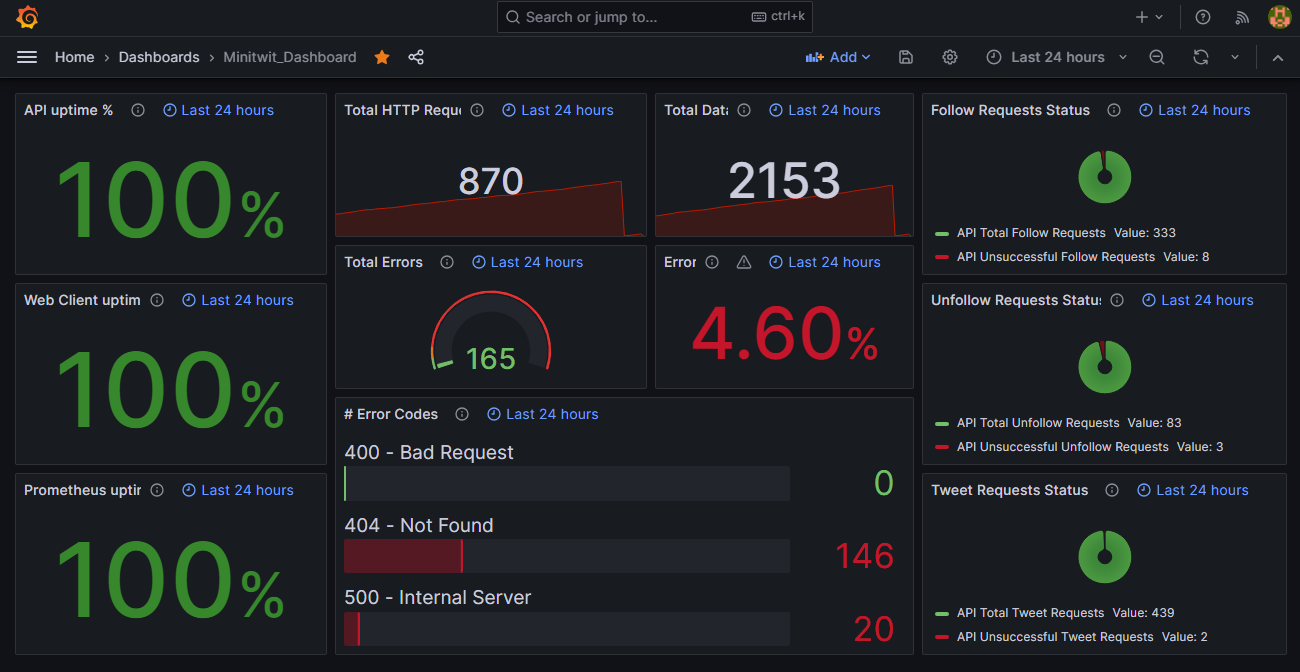
\includegraphics[width=0.8\textwidth]{images/monitor_good.png}
    \caption{Minitwit\_Dashboard - API Monitoring}
    \label{fig:monitor_good}
\end{figure}

The key metrics are categorised and displayed as follows:

\textbf{Total HTTP requests and Database accesses}, \textbf{Total Errors and Error Ratio}, \textbf{Error code distribution} of the total errors, and \textbf{Specific user request success/failure} (follow, unfollow, tweet). 

Additionally, the visualisation shows the uptime percentage of the API, Web Client, and Prometheus, which is derived from predefined Prometheus metrics.

\subsubsection*{Log Aggregation Techniques}
For logging we have used a setup with Promtail, Loki and Grafana. Initially we went for an ELK stack, however after not being able to get it to work and discussing whether it was necessary to do it with that stack, we searched for alternatives and used a setup with Grafana which was already a part of our tech stack. At first this did not work, but when we added Prometheus' AlertManager it worked. The job of AlertManager is to remove duplicate log entries and route them to the correct receiver.

Our techniques included logging general activities of the system with the purpose gaining of an insight into how the system was being used although this was not super useful in our context, but could have proven pivotal as an auditing mechanism if we had experienced database specific issues. This happened on one of our log levels, namely INFO. We also had a level for errors and logged all errors in our system. When we noticed we had a concerning amount of errors of the same type, we created a dashboard view for the specific error. This setup can be seen in figure \ref{fig:logging}

\begin{figure}[H]
    \centering
    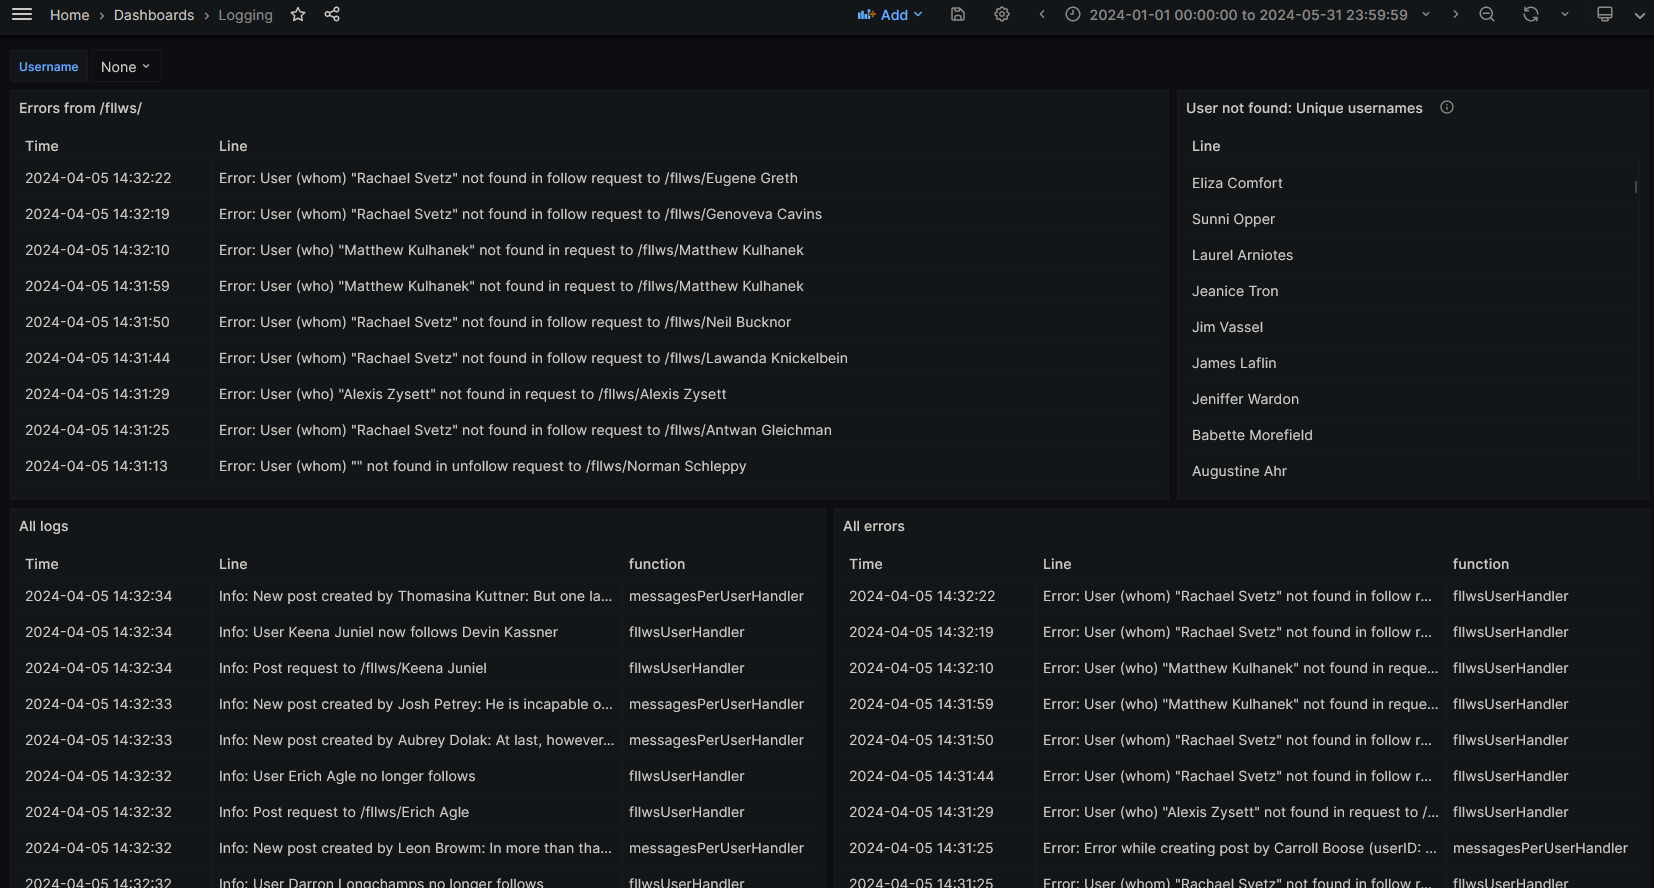
\includegraphics[width=\textwidth]{images/logging.png}
    \caption{Grafana dashboard of logs.}
    \label{fig:logging}
\end{figure}


\subsection{Security Assessment}
In our efforts to ensure the security of the ITU-MiniTwit system, we have utilized various tool for risk identification, such as Snyk, Metasploit and SonarCloud. To assess the security state of our system we have identified threats and provide a risk analysis.

\subsubsection*{Risk Identification}
Our primary asset is the ITU-MiniTwit web application, which includes several components, such as the frontend, backend, database and the associated cloud infrastructure.

One of the most common vulnerabilities for web applications involves injecting malicious SQL statements. Other similar threat sources consists of cross-site scripting (XSS) or misconfiguration, e.g. incorrectly configured servers, databases or applications that can expose vulnerabilities.

From this we can construct several risk scenarios:

\begin{multicols}{2}
    \begin{itemize}
        \item \textbf{Scenario 1}: An attacker performs SQL injection on the web application to download sensitive user data.
        \item \textbf{Scenario 2}: An attacker exploits a cross-site scripting vulnerability to steal session cookies and impersonate users.
        \item \textbf{Scenario 3}: An attacker exploits a misconfiguration of the web server allowing unauthorized access to system resources.
        \item \textbf{Scenario 4}: A developer with legitimate access exposes sensitive data or sabotages the system, either intentionally or accidentally.
    \end{itemize} 
\end{multicols}

%"https://documents.ncsl.org/wwwncsl/Task-Forces/Cybersecurity-Privacy/IBM_Ponemon2017CostofDataBreachStudy.pdf" ved vi at "however we know from (kilde) that the the most common way to discover security failures is when a security incident happens.

\subsubsection*{Risk Analysis}
To analyze the identified risks we evaluate using a risk matrix to prioritize them based on their likelihood and impact.

\begin{table} [H]
    \centering
    \begin{tabular}{|c||c|c|c|}
        \hline
        Risk Scenario & Likelihood & Impact & Priority \\ \hline\hline
        SQL Injection & Low & High & Medium\\ \hline
        XSS & Low & Medium & Low \\ \hline 
        Misconfiguration & Medium & High & High \\ \hline 
        Developer error & Low & High & Medium \\ \hline
    \end{tabular}
    \caption{Risk matrix based on identified risks.}
    \label{tab:risk_matrix}
\end{table}

To mitigate the risk scenarios the following strategies are employed:
\begin{itemize}
    \item \textbf{Static code analysis}: The likelihood of our risk scenarios is covered in part by SonarCloud that has security rules setup, which analyzes the source code and allows detecting SQL Injection and XSS. %https://docs.sonarsource.com/sonarcloud/digging-deeper/security-related-rules/
    \item \textbf{Secrets}: To minimize the risk of exposing sensitive data, we use secrets in Docker swarm, GitHub and CircleCI. 
    \item \textbf{Automation}: Automatic configuration e.g. using tools like Vagrant or Terraform ensures we avoid misconfigurations.
\end{itemize}

\subsubsection*{Security Hardening}
%HTTPS
%Docker secrets

Other security measures that we have in place are using https on our domains and using Docker secrets for sensitive data such as our database connection string.\\

Our HTTPS certificate is obtained through CertBot. However, due to difficulties with the standard HTTP validation method, especially concerning load balancers as described in the article "How To Acquire a Let's Encrypt Certificate Using DNS Validation with acme-dns-certbot," \cite{certbotDigitalOceanIssues} we opted for an alternative approach. We used the acme-dns-certbot tool \cite{acmedns}, which interfaces CertBot with a third-party DNS server for validation instead of HTTP. This method is especially beneficial for issuing certificates for individual servers behind a load balancer, where traditional HTTP certificate validation would require setting validation files on each server.

\subsection{Scaling and Upgrade Strategy}
%docker swarm
From our monitoring dashboard we could at one point identify several API crashes on our single Digital Ocean node due to 100\% CPU usage. As a method to regain availability by removing the single-point-of-failure and reach a generally more robust service, we chose to employ scaling and replication through Docker Swarm.

\subsubsection*{Docker Swarm}
We chose Docker Swarm as our container orchestration platform because it is included by default with Docker and is simpler to use compared to alternatives like Kubernetes and OpenShift. Docker Swarm allowed us to set up a cluster consisting of manager and worker nodes, effectively creating a distributed system. In this setup, worker nodes run our stateful services, API and web client, independently, while the manager node handles service scheduling across the nodes using the routing mesh, Docker Swarm's built-in load balancing mechanism, and maintains the swarm state.

We first deployed the Docker Swarm as a separate cluster beside our single-node production server in Digital Ocean to ensure a transition that would not disrupt our live server. For each service, including our API, we added an additional replica in order to distribute the workload across multiple containers.

However, as the inherent load balancer, the routing mesh, of Docker Swarm is rather low-level, in which it from-the-shelf only redirects traffic to replicas when a node is “unhealthy”, or dead, we opted for a dedicated load balancer to complement the routing mesh by employing a more sophisticated traffic distribution. Simply redirecting traffic when a node is crashed  that initiated the whole focus on scaling and replication.

\subsubsection*{Nginx}
We chose to utilise Nginx as both reverse proxy and load balancer. This involved adding a new droplet in our Digital Ocean project outside the swarm to run an instance of Nginx, which we configured to handle a more sophisticated traffic distribution between the replicated services.

To configure Nginx, we separated the configuration files into two parts, one for the API and one for the web client. The configuration file for the API includes an upstream block that lists the IP addresses of the replicas in the swarm cluster along the API ports, allowing Nginx to direct traffic to the specified instances. Additionally we added server blocks for HTTP and HTTPS traffic, effectively redirecting all HTTP traffic to HTTPS. Similarly, the configuration file for the web client follows the same pattern but includes the IP addresses and service ports of the web client in the upstream block instead. See appendix \textcolor{red}{X} for the configuration file of the API service.


\subsection{AI Tools Utilized}
To automate the production of easy or recurring code such as a new prometheus monitoring metric, generating skeleton code, code completion and helping us gaining a high-level understanding of the ITU-MiniTwit system, Microsoft Copilot was used by multiple developers. It was quite bad at guessing the intended implementation logic of new features.